\chapter{Desarrollo}
\label{cap:desarrollo}

En este capítulo se va a llevar a cabo el estudio del arte relativo a este proyecto y se van a comentar el proceso de desarrollo realizado para conseguir los objetivos establecidos.

\section{Estudio del arte}

El estudio del arte debe hacerse por partida doble. Debe estudiarse el estado en el que se encuentra Android y a parte, los \texit{CBIR} en dicha plataforma.\\

\subsection{Estado arte Android}

Por la parte de la lógica no hay ningún tipo de misterio, ya que tratamos con Java y XML, cosas que apenas cambian y ya se tienen muy estudiadas y asimiladas, por lo que no es necesario un gran estudio de esta parte.\\

Lo que si hay que tener en cuenta es el desarrollo de interfaces de usuario. Este es un tema muy importante, ya que aunque la aplicación funcione correctamente y presente unas novedades increíbles, un mal diseño de interfaz puede provocar su abandono por parte de los usuarios. Resulta natural dedicar un tiempo de investigación a esta parte.\\

\subsubsection{Material design}
Al realizar cualquier búsqueda sobre diseño de interfaces en Android nos encontramos con \textit{Material design}, que se trata de una guía integral para el diseño visual, de movimientos y de interacción en distintas plataformas y dispositivos. Presenta una gran serie de nuevos elementos y novedades. Actualmente es el estándar de Android. Debido a esto, se debe seguir \textit{Material design} a la hora de realizar una interfaz.

\begin{figure}[H] %con el [H] le obligamos a situar aquí la figura
\centering
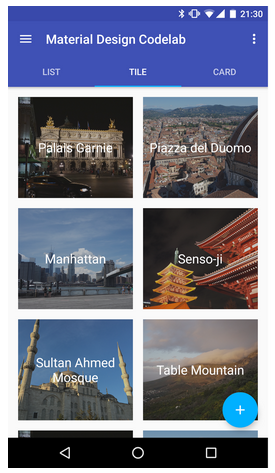
\includegraphics[scale=0.5]{imagenes/desing1.png}  %el parámetro scale permite agrandar o achicar la imagen. En el nombre de archivo puede especificar directorios
\label{design1}
\caption{Ejemplo de Material Design 1}
\end{figure}

\begin{figure}[H] %con el [H] le obligamos a situar aquí la figura
\centering
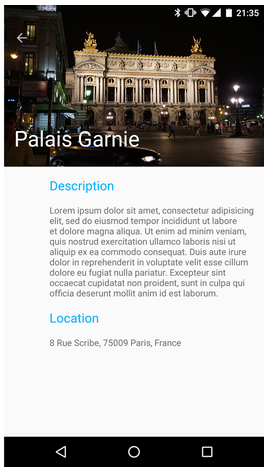
\includegraphics[scale=0.5]{imagenes/desing2.png}  %el parámetro scale permite agrandar o achicar la imagen. En el nombre de archivo puede especificar directorios
\label{design1}
\caption{Ejemplo de Material Design 2}
\end{figure}

Tras un estudio preliminar de \textit{Material design} se procedió a estudiar con más detalle dos elementos. Estos son \textit{floating action button}, \textit{Bottom Navigation} y \textit{Glide}.

\subsubsection{Floating action button}

Un \textit{Floating action button} representa la acción principal en una aplicación. Normalmente se encuentra en forma de un icono en circular que se encuentra flotando sobre la interfaz de usuario, cambia de color al pulsar y se eleva al seleccionar. Cuando se presiona, puede contener más acciones relacionadas.\\

En mi caso he utilizado la implementación usada por \textit{Clans}, el código fuente se puede encontrar en su \href{https://github.com/Clans/FloatingActionButton}{repositorio}

\begin{figure}[H] %con el [H] le obligamos a situar aquí la figura
\centering
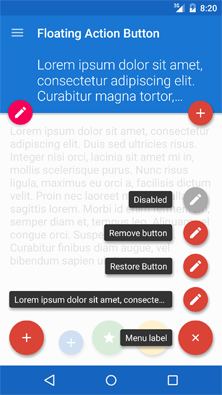
\includegraphics[scale=0.5]{imagenes/fab.png}  %el parámetro scale permite agrandar o achicar la imagen. En el nombre de archivo puede especificar directorios
\label{fab}
\caption{Ejemplo Floating action button}
\end{figure}

\subsubsection{Bottom Navigation}

Los \textit{Bottom Navigation} nos proporciona una navegación rápida entre las vistas de nivel superior de una aplicación. Está diseñado principalmente para su uso en dispositivos móviles. Las pantallas más grandes, como el escritorio, pueden lograr un efecto similar usando la navegación lateral. Por ejemplo, el tratamiento compacto "rail" muestra los iconos de navegación de forma predeterminada.\\

En mi caso he utilizado la implementación usada por \textit{sephiroth74}, el código fuente se puede encontrar en su \href{https://github.com/sephiroth74/Material-BottomNavigation}{repositorio}\\

\begin{figure}[H] %con el [H] le obligamos a situar aquí la figura
\centering
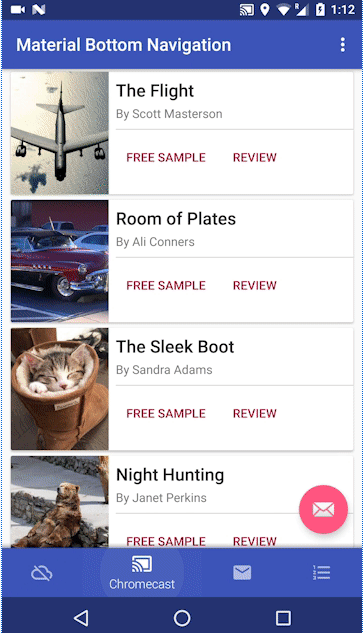
\includegraphics[scale=0.5]{imagenes/mbottom.png}  %el parámetro scale permite agrandar o achicar la imagen. En el nombre de archivo puede especificar directorios
\label{mbottom}
\caption{Ejemplo Bottom Navigation}
\end{figure}

\subsubsection{Glide}

Se trata de un marco de trabajo rápido y eficiente de código abierto que se encarga de la gestión de imágenes, agrupando la decodificación de medios, la gestión de memoria y el almacenamiento de cache en disco mediante una interfaz simple y sencilla de utilizar.\\

Actualmente se encuentra recomendada por \textit{Google}, está desarrollada por \textit{Bump Technologies}, y se puede consultar en el enlace de su \href{https://github.com/bumptech/glide}{repositorio}\\


\begin{figure}[H] %con el [H] le obligamos a situar aquí la figura
\centering
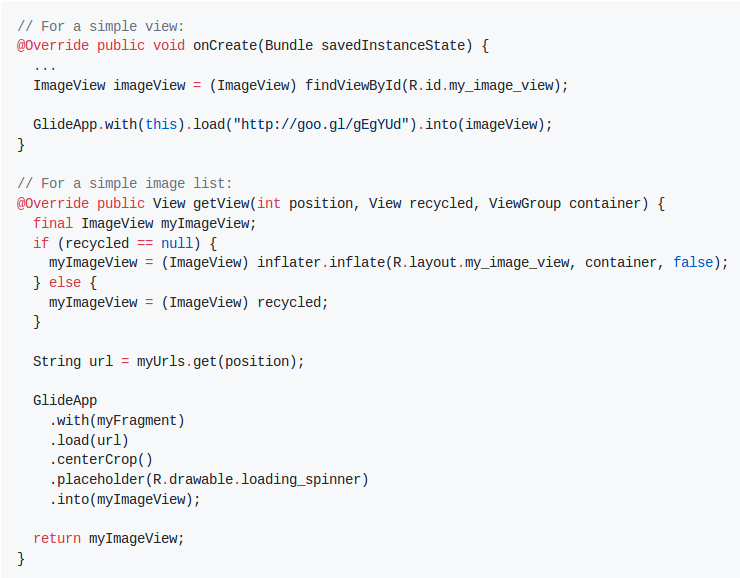
\includegraphics[scale=0.5]{imagenes/glide.png}  %el parámetro scale permite agrandar o achicar la imagen. En el nombre de archivo puede especificar directorios
\label{glide}
\caption{Ejemplo de uso de Glide}
\end{figure}

En nuestro caso es ideal, ya que nos proporciona una manera sencilla de trabajar con imágenes y a su vez, nos permite utilizar movimientos de desplazamiento scroll de una manera simple, lo que nos posibilita centrarnos en la manera en la que queremos representar las imágenes.

\subsection{Estado CBIR Android}

Lo primero que podemos encontrar es información abundante sobre CBIR en computadores, pero en nuestro caso no nos es necesaria, ya que partimos de uno previo, \textit{Java Multimedia Retrieval}, que cuenta con todo lo que necesitamos sobre este tipo de sistemas. Aunque siempre es interesante estar al día en estos asuntos.\\

Por lo que vamos a centrarnos en los CBIR desarrollados exclusivamente para sistemas Android, aunque sobre este tema concreto, no hay demasiada información.

\subsubsection{Content based image retrieval for mobile systems}

En esta ocasión nos encontramos ante un artículo escrito por \textit{P Jeyanthi} profesor asociado del departamento de tecnologías de la información de la universidad Sathyabama, Rajiv Gandhi Salai, India.\\

En el artículo se habla sobre un enfoque para la realización de la extracción de características basadas en textura por la co-ocurrencia de nivel de gris y la matriz de color basado en la extracción de características por color vector de concurrencia. La mayor parte del artículo se centra en el cálculo de descriptores, cosa que como se ha mencionado antes, a nosotros no nos es relevante. Por otro lado podemos ver un poco de la interfaz, lo que si nos interesa, aunque comprobamos de que se trata de una interfaz muy pobre, ya que se concentran en el cálculo de descriptores más que en la representación de los resultados.


\begin{figure}[H] %con el [H] le obligamos a situar aquí la figura
\centering
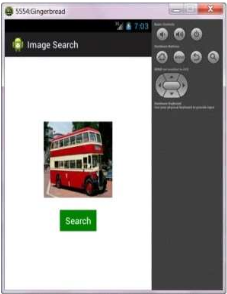
\includegraphics[scale=0.6]{imagenes/articulo11.png}  %el parámetro scale permite agrandar o achicar la imagen. En el nombre de archivo puede especificar directorios
\label{articulo11}
\caption{Interfaz CBIR for mobile systems 1}
\end{figure}

\begin{figure}[H] %con el [H] le obligamos a situar aquí la figura
\centering
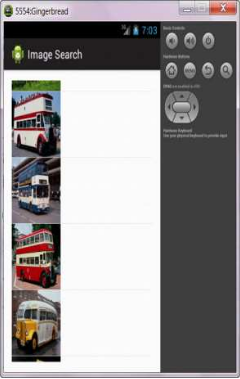
\includegraphics[scale=0.6]{imagenes/articulo12.png}  %el parámetro scale permite agrandar o achicar la imagen. En el nombre de archivo puede especificar directorios
\label{articulo11}
\caption{Interfaz CBIR for mobile systems 2}
\end{figure}

Otro de los aspectos que nos interesan es el tiempo de cómputo y el consumo de recursos, pero no se hace ningún tipo de referencia a estos aspectos en el artículo.\\

Tras realizar un estudio del estado del arte de los CBIR en Android podemos llegar a la conclusión de que se tratan de sistemas que han sido poco explotados en dicha plataforma, y lo más importante, el usuario medio no conoce de su existencia, por lo que este proyecto cubre un espacio de mercado que se encuentra desocupado.\\

\section{Proceso de desarrollo}

En esta sección vamos a detallar los distintos elementos que componen el proyecto con un nivel de detalle suficiente para dar una visión global del proyecto y entender cada uno de sus componentes.\\

Como visión global podemos ver la aplicación como una única actividad que va cambiando el fragment que se muestra en pantalla, cada fragment se encarga de sus propias tareas, dejando a la actividad encargándose únicamente de cambiar fragments y otras cosas triviales.

\subsection{Paquetes}

Vamos a comenzar hablando de los distintos paquetes de los que se compone el proyecto.

\begin{figure}[H] %con el [H] le obligamos a situar aquí la figura
\centering
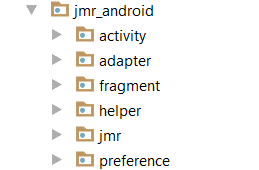
\includegraphics[scale=0.9]{imagenes/paquetes.png}  %el parámetro scale permite agrandar o achicar la imagen. En el nombre de archivo puede especificar directorios
\label{paquetes}
\caption{Paquetes del proyecto}
\end{figure}

\subsubsection{Activity}

En él se encuentran las activities que forman parte del proyecto. En este caso solo forma parte de él una única actividad, \textit{MainActivity} que es la encarga de gestionar la aplicación.

\subsubsection{Adapter}

Formado por \textit{GalleryAdapter} y \textit{ViewPagerAdapter}. El primero se encarga de renderizar las imágenes para su correcta visualización, mientras que el segundo se encarga se usa para permitir que podamos interactuar con las imágenes.

\subsubsection{Fragment}

En este paquete se encuentran los distintos framgents de los que se componen el proyecto, un total de 4. Los tres primeros se corresponden a cada una de las opciones del menú inferior de la aplicación, mientras que el último se encarga de que podamos interactuar con las imágenes al pulsar sobre ellas, aportándonos información.

\subsubsection{Helper}

Formado por clases que se encargan de \textit{ayudar} al resto para que su funcionamiento sea el esperado. Entre algunos de los miembros de este paquete destacan \textit{DBHelper}, que se encarga de la gestión de la base de datos y \textit{GalleryHelper}, encargado de la gestión de la galería del usuario.

\subsubsection{JMR}

Paquete en el que se encuentra todo lo relacionado con el cálculo de descriptores y la organización de sus resultados. A su vez cuenta con clases como \textit{HMMDImage} que se encarga de pasar una imagen en el espacio de color \textit{RGB} al espacio de color \textit{HMMD}. Esto se explicará con detalle en el próximo apartado

\subsubsection{Preference}

En este paquete se encuentran una serie de clases que representan los elementos que se encuentran en la sección adicional de la aplicación. Son necesarios para que esta responda como es esperada, ya que \textit{Android} no nos proporcionaba por defecto lo que buscábamos.

\subsection{Clases}

Una vez que se ha terminado de hablar de los paquetes, es hora de hablar de cada clase individualmente. Al igual que en el caso anterior, lo haremos con cierto nivel de detalle, sin entrar en cuestiones demasiado técnicas.\\

Comenzaremos mostrando los diagramas de clases individuales de cada proyecto, para una mejor compresión de las clases.\\

\subsection{Diagramas de clases}

\begin{figure}[H] %con el [H] le obligamos a situar aquí la figura
\centering
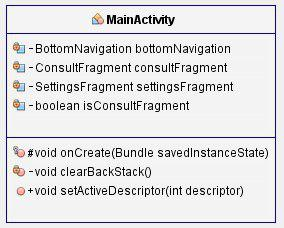
\includegraphics[scale=0.6]{imagenes/diagrama1.jpg}  %el parámetro scale permite agrandar o achicar la imagen. En el nombre de archivo puede especificar directorios
\label{diagrama1}
\caption{Diagrama clase paquete Activity}
\end{figure}

\begin{figure}[H] %con el [H] le obligamos a situar aquí la figura
\centering
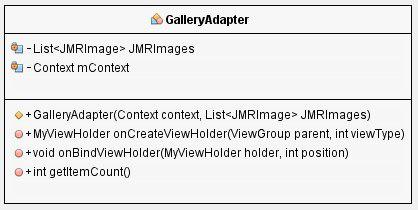
\includegraphics[scale=0.6]{imagenes/diagrama2.jpg}  %el parámetro scale permite agrandar o achicar la imagen. En el nombre de archivo puede especificar directorios
\label{diagrama2}
\caption{Diagrama clase paquete Adapter}
\end{figure}

\begin{figure}[H] %con el [H] le obligamos a situar aquí la figura
\centering
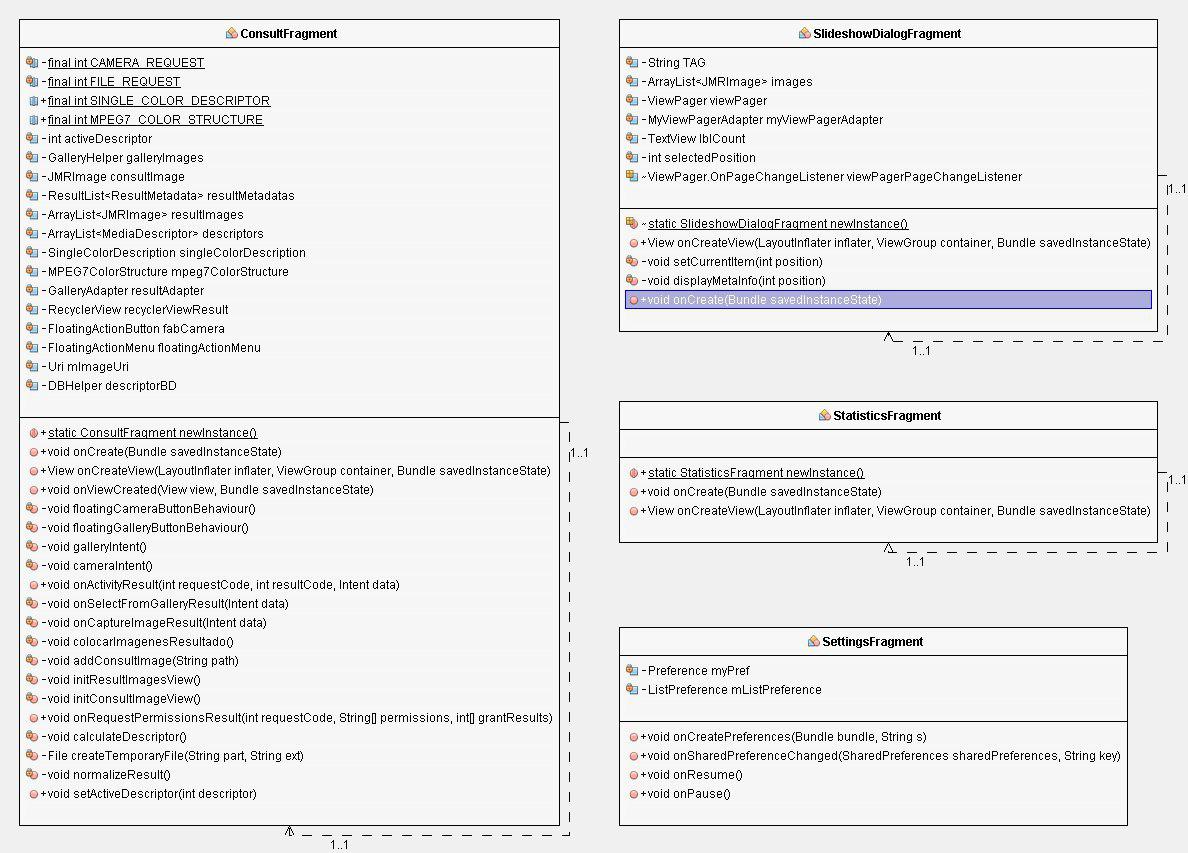
\includegraphics[scale=0.6]{imagenes/diagrama3.jpg}  %el parámetro scale permite agrandar o achicar la imagen. En el nombre de archivo puede especificar directorios
\label{diagrama3}
\caption{Diagrama clase paquete Fragment}
\end{figure}

\begin{figure}[H] %con el [H] le obligamos a situar aquí la figura
\centering
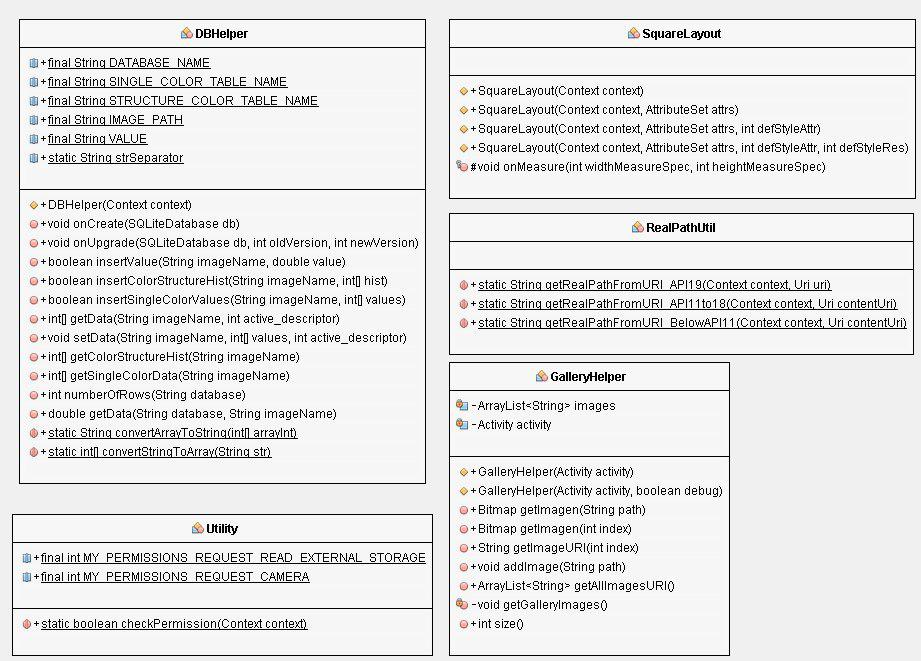
\includegraphics[scale=0.6]{imagenes/diagrama4.jpg}  %el parámetro scale permite agrandar o achicar la imagen. En el nombre de archivo puede especificar directorios
\label{diagrama4}
\caption{Diagrama clase paquete Helper}
\end{figure}

\begin{figure}[H] %con el [H] le obligamos a situar aquí la figura
\centering
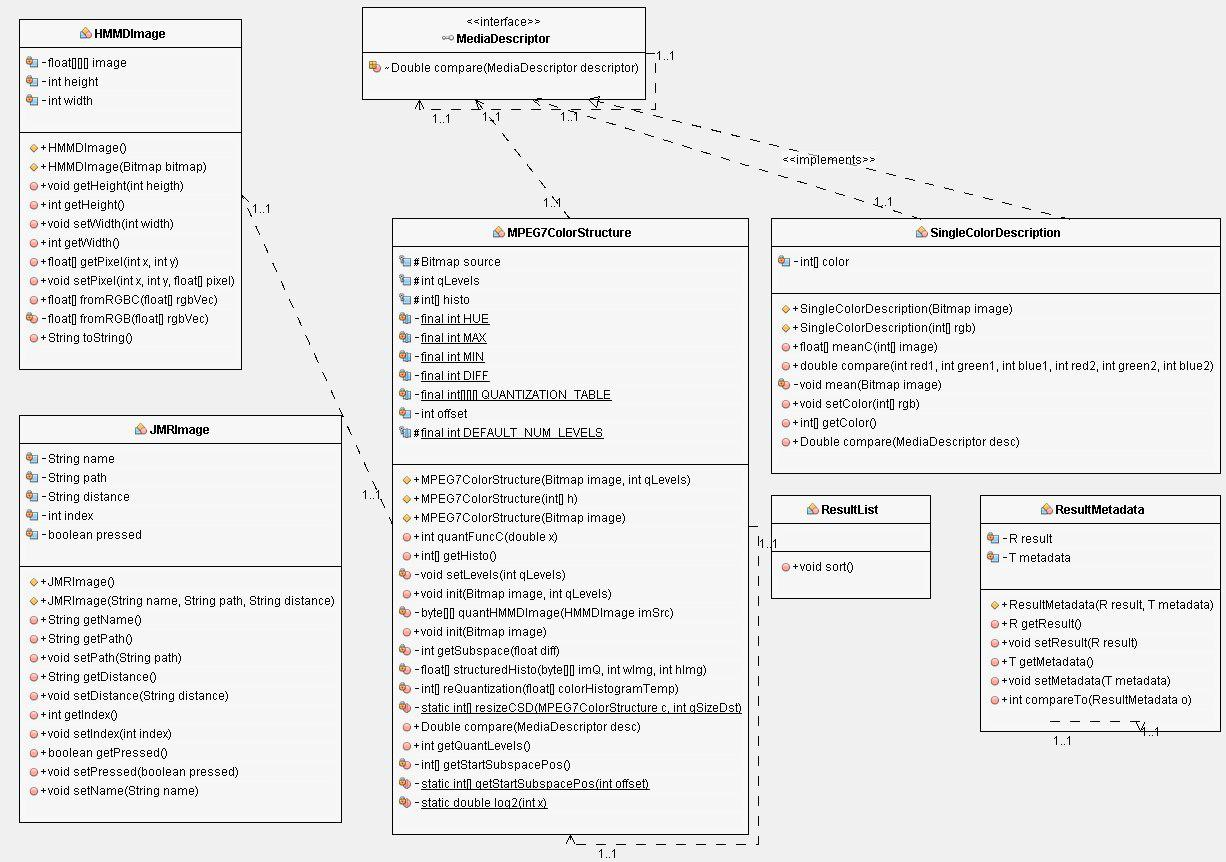
\includegraphics[scale=0.6]{imagenes/diagrama5.jpg}  %el parámetro scale permite agrandar o achicar la imagen. En el nombre de archivo puede especificar directorios
\label{diagrama5}
\caption{Diagrama clase paquete JMR}
\end{figure}

\begin{figure}[H] %con el [H] le obligamos a situar aquí la figura
\centering
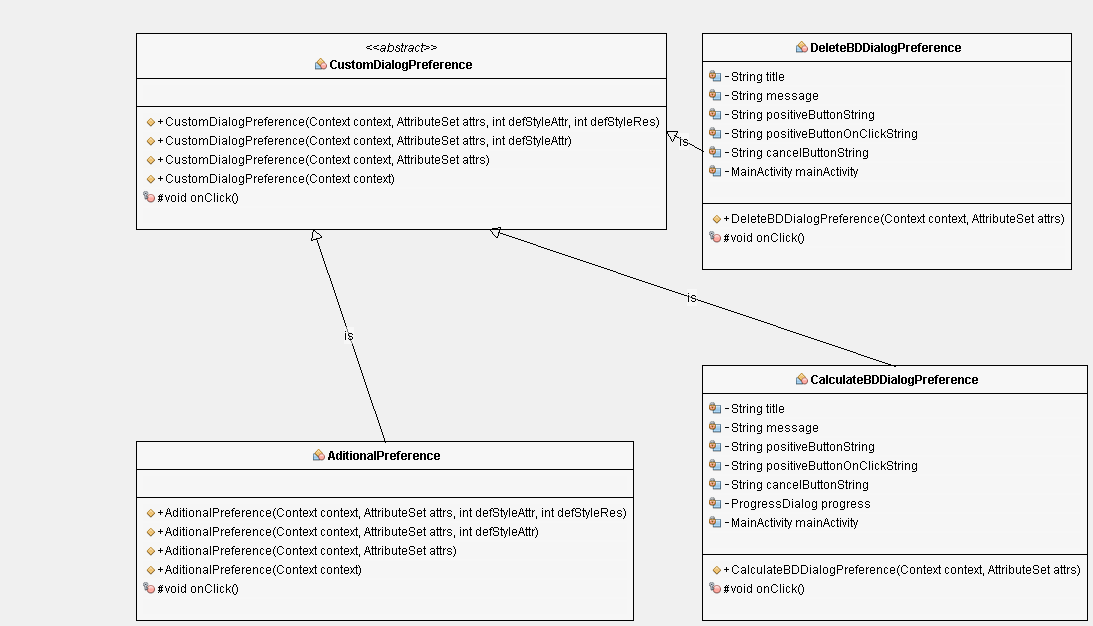
\includegraphics[scale=0.4]{imagenes/diagrama6.png}  %el parámetro scale permite agrandar o achicar la imagen. En el nombre de archivo puede especificar directorios
\label{diagrama6}
\caption{Diagrama clase paquete Preference}
\end{figure}


\subsubsection{MainActivity}

Es la única clase actividad, \textit{Activity}, del proyecto. Se encarga de instanciar e iniciar las 3 clases \textit{Fragment} que se corresponden a cada una de las opciones del menú inferior. A su vez, se ocupa de la comunicación entre \textit{Fragments}, necesaria para un correcto funcionamiento de la aplicación, y también se ocupa de gestionar la memoria, para evitar que la aplicación ocupe demasiados recursos. Esto se consigue controlando la cola de \textit{Fragments} de la aplicación.

\subsubsection{GalleryAdapter}

Esta clase se encarga de \textit{hinchar}, \textit{inflate}, un fichero XML llamado gallery\_thumbnail.xml, en el cuál se colocan las imágenes, una por cada instancia del fichero, y a su vez, se encarga de reenderizar las imágenes. Se puede decir, que esta clase se encarga de colocar todas las imágenes y nos permite interactuar con ellas a través de eventos.

\subsubsection{ConsultFragment}

Clase de tipo \textit{Fragment} que puede considerarse como el núcleo del proyecto.\\

En ella se inicializa su propia interfaz, al igual que el resto de sus clases \textit{Fragment} hermanas. Garantiza que el usuario pueda elegir la imagen consulta tanto de la cámara como de la galería, estas imágenes se van acumulando en la parte superior de la pantalla, pudiendo moverse realizando un movimiento de scroll. También gestiona los permisos, ya que es aquí donde se encuentran los métodos que requieren de ellos para poder desempeñar correctamente su función.\\

Todos los cálculos de descriptores son realizados aquí, consultado previamente si los valores a calcular se encuentran en la base de datos y actuando en consecuencia. Para estos cálculos se utilizan las clases que se encuentran en el paquete JMR. Las imágenes resultantes de una consulta, imágenes resultado, se colocan justo debajo de las imágenes consulta, en cuatro columnas, pudiendo realizar un movimiento de scroll en caso de que no cupiesen todas en la pantalla del dispositivo.

\subsubsection{SettingsFragment}

Esta clase se encarga de gestionar el apartado de opciones de la aplicación. Permite al usuario elegir con que descriptor desea realizar las consultas, entre otras cosas. Básicamente, a través de eventos recoge las acciones del usuario y se las transmite a otras clases, en caso de ser necesario, usando la clase \textit{MainActivity}.\\

Un ejemplo de esto es cuando el usuario decide cambiar el descriptor activo. En esa ocasión, esta clase notifica a \textit{ConsultFragment} utilizando a \textit{MainActivity}

\subsubsection{SlideshowDialogFragment}

Esta clase, junto con su clase interna adapter, \textit{MyViewPageAdapter}, nos proporciona los métodos necesarios para que, cuando pulsemos una imagen, esta aparezca ocupando toda la pantalla y a su vez, nos muestra información sobre ella. Esta información es el número de imagen que ocupa del total, imagen 5 de 400, y la distancia de la imagen consulta, un valor entre 0 y 1 que nos indica como de parecidas son las imágenes entre si, siendo 0 iguales y 1 totalmente distintas.

\subsubsection{Fragment sobre nosotros}

Poner licencias, que hable un poco del proyecto.
 
\subsubsection{DBHelper}

Clase encargada de la gestión de la base de datos. Cuenta con métodos para crearla, alterarla y destruirla. Cuando se están realizando los cálculos de los descriptores, se consulta la base de datos a través de los métodos de esta clase, para comprobar si el valor que se desea calcular se encuentra en ella, o en caso contrario, introducirlo. Esta base de datos es de tipo relacional.

\subsubsection{GalleryHelper}

Se encarga de gestionar todas las imágenes disponibles en el dispositivo del usuario, como es natural pensar, requiere de permisos por parte de él. Dispone de todo tipo de métodos para obtener las imágenes, y para minimizar el consumo de recursos lo único que se mantiene en memoria es la ruta de las imágenes, \textit{path}. Cuando es necesario cargar una imagen, se hace en base a su ruta, lo que evita tener todas las imágenes en memoria, un escenario que sería imposible.

\subsubsection{RealPathUtil}

Clase que se ocupa de tratar la ruta o \textit{path} de las imágenes, tarea que puede resultar trivial, pero no lo es.

\subsubsection{SquareLayout}

En esta ocasión, esta clase extiende de \textit{RelativeLayout} y se encarga de representar una imagen de manera cuadrada en un \textit{grid view}, es decir, en las 4 columnas de las que hablábamos previamente.

\subsubsection{Utility}

Se encarga de gestionar los permisos que necesitan el resto de clases para actuar correctamente. Cuando una clase requiere cualquier tipo de permiso se pone en contacto con ella y actúa en consecuencia.

\subsubsection{HMMDImage}

Dado que el descriptor \textit{MPEG7ColorStructure} necesita que la imagen en el espacio de color HMMD, esta clase se encarga de dicha tarea. Utiliza una imagen en espacio de color RGB y la transforma HMMD, con una serie de operaciones matemáticas no muy complejas.

\subsubsection{JMRImage}

Siempre que nos referimos a imagen, nos referimos a esta clase. Cuenta con todo lo necesario para garantizar que el consumo de memoria sea lo mínimo posible, como se ha comentado anteriormente. Simplemente guarda información sobre la imagen, pero no a la propia imagen. Esta información es utilizada a la hora de cargar la imagen, y de añadirle más nivel de detalle, tal que el número de la imagen respecto a las demás o su distancia a la imagen consulta, en caso de que se trate de una imagen resultado.

\subsubsection{MPEG7ColorStructure}

Clase que representa al descriptor de mismo nombre y que utiliza el histograma de una imagen en espacio de color HMMD, que posteriormente se comparará con el resto de histogramas del resto de las imágenes para ver cuan parecidas son entre ellas.

\subsubsection{ResultList}

Extiende de \textit{LinkedList}, en la cual se almacenaran los objetos de la clase \textit{ResultMetadata}.

\subsubsection{ResultMetada}

Clase parametrizable que representa el resultado de una descriptor. Contiene dos atributos que pueden ser de cualquier tipo, en este caso dichos atributos son de tipo \textit{String}, que representa la ruta o \textit{path} de la imagen y un \textit{Double}, que representa la distancia entre dos imágenes, como de parecidas son en un valor que va desde 0 a 1.\\

A su vez implementa la interfaz \textit{Comparable}, de esta manera garantizamos de que se disponga de un método para comparar distintos \textit{ResultMetada}

\subsubsection{SingleColorDescriptor}

Representa al otro descriptor disponible en el proyecto. En este caso se calcula el color medio de una imagen en espacio de color RGB, recorriendo la imagen píxel a píxel.

\subsubsection{AditionalFragmet}

Clase que extendiende de \textit{PreferenceFragmentCompat} e implementa la interfaz \textit{SharedPreferences.OnSharedPreferenceChangeListener}. Esta clase representa la

\subsection{Código nativo}

Como se ha comentado en la memoria, algunas partes del código han sido implementadas en código nativo utilizando \textit{Android nkd}. Solo ha sido implementado un poco del proyecto por dos razones:

\begin{itemize}
\item Carencia de tiempo y complejidad: Dado que he estado realizando prácticas a media jornada en una empresa y a la dificultad de encontrar la resolución a algunas dudas, me ha sido imposible aumentar la cantidad de código nativo del proyecto. Aunque, se va a tener muy en cuentra como trabajo futuro del proyecto.

\item Malos resultados: En algunas ocasiones, al implementar algunas funciones sencillas en código nativo, se obtenían unos tiempos peores que empleando la misma función implementada en Java. Por lo que como trabajo futuro, se investigará el motivo con mas detalle. 

\end{itemize} 
